% Professional TikZ figures — data from verified experiment artifacts
% ALIGN01/03, GEO01, TRENDS01, STAT01, INTL01 (no fabricated values)
\usepackage{pgfplots}
\pgfplotsset{compat=1.18}
\usepgfplotslibrary{groupplots,statistics}
\usetikzlibrary{patterns,positioning,calc}

% ---- Shared style (publication-grade, high-contrast scientific palette) ----
\definecolor{sgBlue}{RGB}{31,119,180}     % Market demand / primary (#1F77B4)
\definecolor{sgTeal}{RGB}{26,125,140}     % Lexical measurement (#1A7D8C)
\definecolor{sgGreen}{RGB}{46,125,50}     % Semantic measurement (#2E7D32)
\definecolor{sgOrange}{RGB}{220,100,20}   % Lexical deficit (#DC6414)
\definecolor{sgRed}{RGB}{195,35,35}       % Semantic deficit / contrast (#C32323)
\definecolor{sgGrey}{RGB}{110,120,130}    % Reference lines, whiskers (#6E7882)
\definecolor{sgLight}{RGB}{240,242,245}   % Subtle grid (#F0F2F5)
\definecolor{sgAxis}{RGB}{140,145,150}    % Axis lines (#8C9196)

\pgfplotsset{
  sg axis/.style={
    axis line style={sgAxis, line width=0.5pt},
    tick style={sgAxis, line width=0.5pt},
    label style={font=\footnotesize, color=black!85},
    tick label style={font=\scriptsize, color=black!75},
    legend style={
      font=\scriptsize,
      draw=sgAxis!50,
      fill=white,
      cells={anchor=west},
      inner sep=3pt,
      /tikz/every even column/.append style={column sep=6pt},
    },
    ymajorgrids=true,
    grid style={sgLight, line width=0.5pt},
    scale only axis,
  },
}
\tikzset{
  sg bar/.style={
    fill=#1,
    draw=#1!80!black,
    line width=0.4pt,
  },
}

% ============================================================
% FIG 1 — Top-10 market skill tokens (ALIGN01 market_top500)
% ============================================================
\newcommand{\FigTopSkills}{%
\resizebox{\linewidth}{!}{%
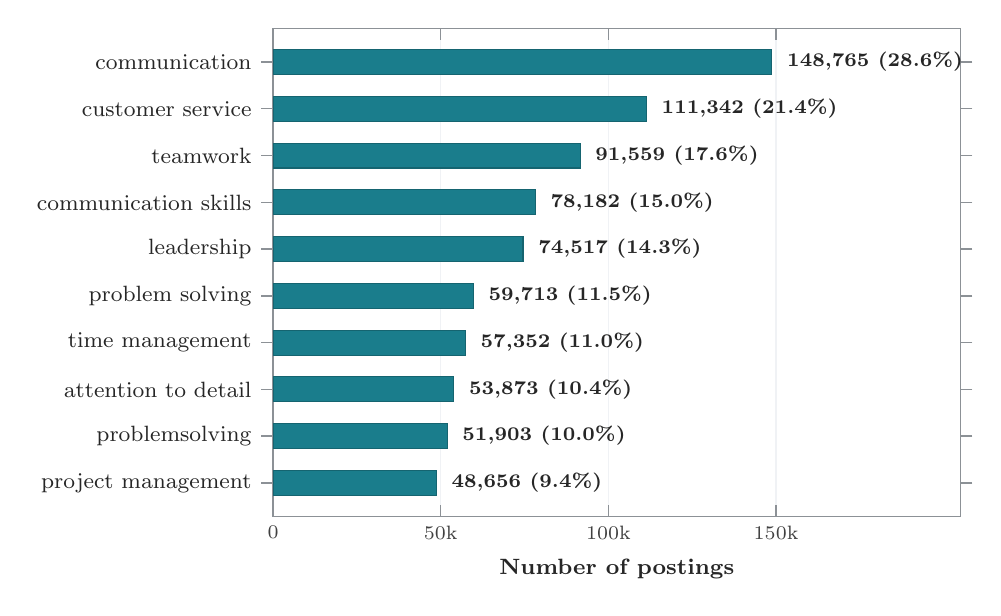
\begin{tikzpicture}
\begin{axis}[
  sg axis,
  xbar,
  bar width=9pt,
  width=0.72\linewidth,
  height=6.2cm,
  symbolic y coords={
    project management,
    problemsolving,
    attention to detail,
    time management,
    problem solving,
    leadership,
    communication skills,
    teamwork,
    customer service,
    communication%
  },
  ytick=data,
  y tick label style={font=\footnotesize, text=black!85, anchor=east},
  xmin=0, xmax=205000,
  xlabel={\textbf{Number of postings}},
  scaled x ticks=false,
  xtick={0,50000,100000,150000},
  xticklabels={0,50k,100k,150k},
  xmajorgrids=true,
  ymajorgrids=false,
  enlarge y limits=0.08,
  nodes near coords,
  nodes near coords align={horizontal},
  every node near coord/.append style={
    font=\scriptsize\bfseries,
    color=black!85,
    anchor=west,
    xshift=2pt
  },
  point meta=explicit symbolic,
]
\addplot[fill=sgTeal, draw=sgTeal!80!black, line width=0.4pt] coordinates {
  (48656,project management) [48,656 (9.4\%)]
  (51903,problemsolving) [51,903 (10.0\%)]
  (53873,attention to detail) [53,873 (10.4\%)]
  (57352,time management) [57,352 (11.0\%)]
  (59713,problem solving) [59,713 (11.5\%)]
  (74517,leadership) [74,517 (14.3\%)]
  (78182,communication skills) [78,182 (15.0\%)]
  (91559,teamwork) [91,559 (17.6\%)]
  (111342,customer service) [111,342 (21.4\%)]
  (148765,communication) [148,765 (28.6\%)]
};
\end{axis}
\end{tikzpicture}%
}%
}

% ============================================================
% FIG 2 — Domain demand / coverage / deficit (ALIGN03)
% ============================================================
\newcommand{\FigGapDemand}{%
\resizebox{\linewidth}{!}{%
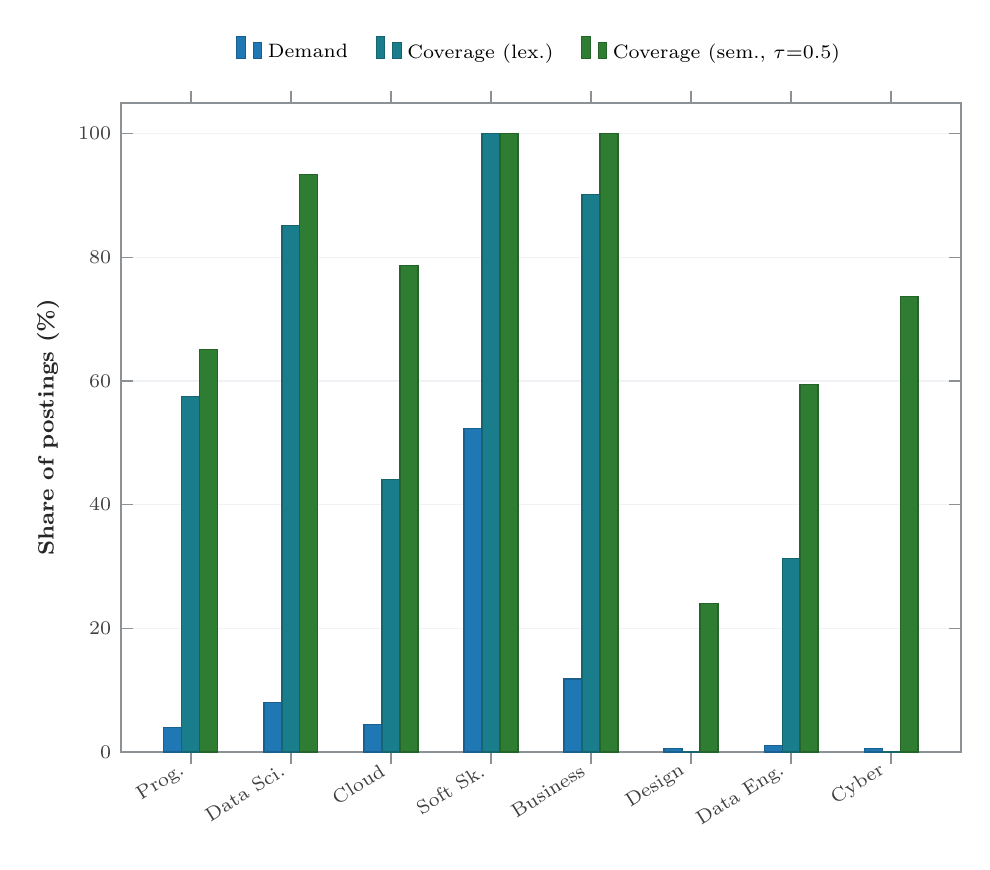
\begin{tikzpicture}
\begin{axis}[
  sg axis,
  ybar,
  bar width=6.5pt,
  width=0.88\linewidth,
  height=0.68\linewidth,
  symbolic x coords={Prog,DataSci,Cloud,Soft,Bus,Design,DataEng,Cyber},
  xtick=data,
  xticklabels={Prog., Data Sci., Cloud, Soft Sk., Business, Design, Data Eng., Cyber},
  x tick label style={rotate=32, anchor=east, font=\scriptsize},
  enlarge x limits=0.10,
  ymin=0, ymax=105,
  ytick={0,20,40,60,80,100},
  ylabel={\textbf{Share of postings (\%)}},
  legend style={
    at={(0.5, 1.04)},
    anchor=south,
    legend columns=-1,
    font=\scriptsize,
    draw=none,
    fill=none,
    /tikz/every even column/.append style={column sep=8pt},
  },
]
\addplot[fill=sgBlue, draw=sgBlue!80!black, line width=0.4pt, bar shift=-6.5pt] coordinates {
  (Prog,3.97)(DataSci,8.04)(Cloud,4.39)(Soft,52.26)(Bus,11.81)(Design,0.60)(DataEng,1.02)(Cyber,0.62)
};
\addlegendentry{Demand}
\addplot[fill=sgTeal, draw=sgTeal!80!black, line width=0.4pt, bar shift=0pt] coordinates {
  (Prog,57.47)(DataSci,85.10)(Cloud,44.06)(Soft,100)(Bus,90.22)(Design,0)(DataEng,31.28)(Cyber,0)
};
\addlegendentry{Coverage (lex.)}
\addplot[fill=sgGreen, draw=sgGreen!80!black, line width=0.4pt, bar shift=6.5pt] coordinates {
  (Prog,65.05)(DataSci,93.36)(Cloud,78.67)(Soft,100)(Bus,100)(Design,24.07)(DataEng,59.50)(Cyber,73.71)
};
\addlegendentry{Coverage (sem., $\tau{=}0.5$)}
\end{axis}
\end{tikzpicture}%
}%
}

\newcommand{\FigGapDeficit}{%
\resizebox{\linewidth}{!}{%
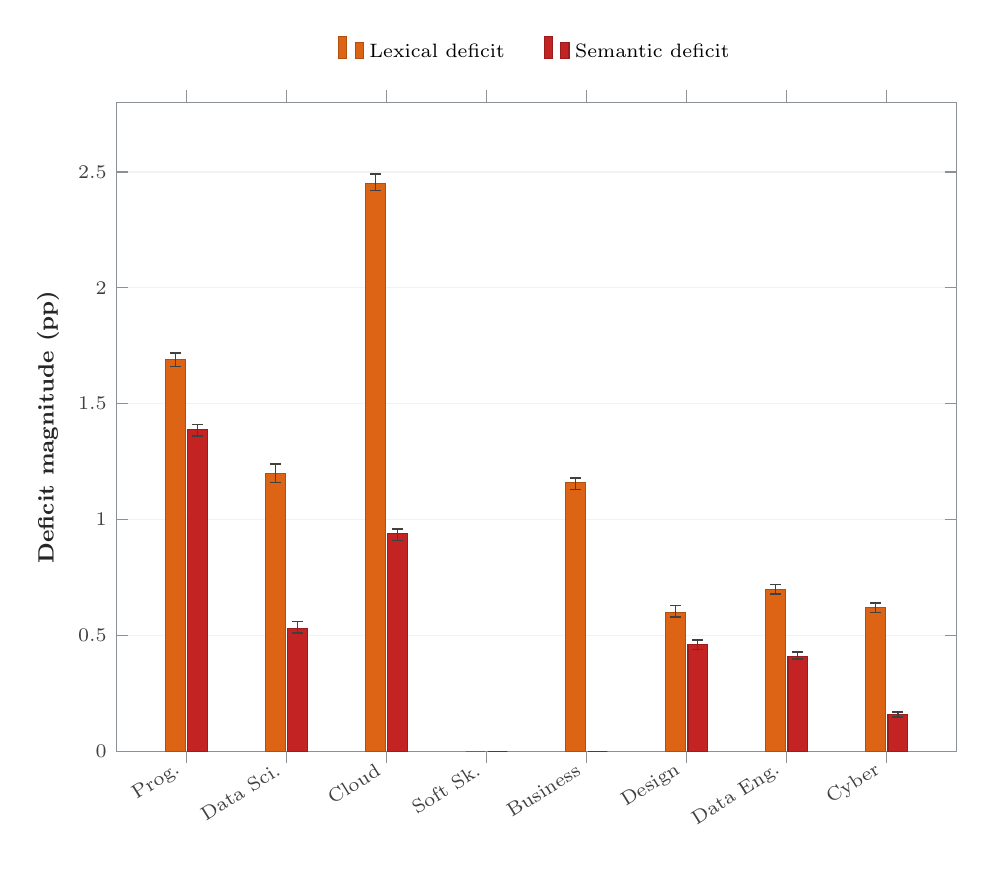
\begin{tikzpicture}
\begin{axis}[
  sg axis,
  ybar,
  bar width=7pt,
  width=0.88\linewidth,
  height=0.68\linewidth,
  symbolic x coords={Prog,DataSci,Cloud,Soft,Bus,Design,DataEng,Cyber},
  xtick=data,
  xticklabels={Prog., Data Sci., Cloud, Soft Sk., Business, Design, Data Eng., Cyber},
  x tick label style={rotate=32, anchor=east, font=\scriptsize},
  enlarge x limits=0.10,
  ymin=0, ymax=2.8,
  ytick={0,0.5,1.0,1.5,2.0,2.5},
  ylabel={\textbf{Deficit magnitude (pp)}},
  legend style={
    at={(0.5, 1.04)},
    anchor=south,
    legend columns=-1,
    font=\scriptsize,
    draw=none,
    fill=none,
    /tikz/every even column/.append style={column sep=12pt},
  },
]
\addplot[fill=sgOrange, draw=sgOrange!80!black, line width=0.4pt, bar shift=-4pt] coordinates {
  (Prog,1.69)(DataSci,1.20)(Cloud,2.45)(Soft,0.00)(Bus,1.16)(Design,0.60)(DataEng,0.70)(Cyber,0.62)
};
\addlegendentry{Lexical deficit}
\addplot[fill=sgRed, draw=sgRed!80!black, line width=0.4pt, bar shift=4pt] coordinates {
  (Prog,1.39)(DataSci,0.53)(Cloud,0.94)(Soft,0.00)(Bus,0.00)(Design,0.46)(DataEng,0.41)(Cyber,0.16)
};
\addlegendentry{Semantic deficit}

% Exact 95% bootstrap CI on Lexical deficit (shifted -4pt)
\draw[black!75, line width=0.6pt] ([xshift=-4pt]axis cs:Prog,1.66) -- ([xshift=-4pt]axis cs:Prog,1.72);
\draw[black!75, line width=0.6pt] ([xshift=-6pt]axis cs:Prog,1.66) -- ([xshift=-2pt]axis cs:Prog,1.66);
\draw[black!75, line width=0.6pt] ([xshift=-6pt]axis cs:Prog,1.72) -- ([xshift=-2pt]axis cs:Prog,1.72);

\draw[black!75, line width=0.6pt] ([xshift=-4pt]axis cs:DataSci,1.16) -- ([xshift=-4pt]axis cs:DataSci,1.24);
\draw[black!75, line width=0.6pt] ([xshift=-6pt]axis cs:DataSci,1.16) -- ([xshift=-2pt]axis cs:DataSci,1.16);
\draw[black!75, line width=0.6pt] ([xshift=-6pt]axis cs:DataSci,1.24) -- ([xshift=-2pt]axis cs:DataSci,1.24);

\draw[black!75, line width=0.6pt] ([xshift=-4pt]axis cs:Cloud,2.42) -- ([xshift=-4pt]axis cs:Cloud,2.49);
\draw[black!75, line width=0.6pt] ([xshift=-6pt]axis cs:Cloud,2.42) -- ([xshift=-2pt]axis cs:Cloud,2.42);
\draw[black!75, line width=0.6pt] ([xshift=-6pt]axis cs:Cloud,2.49) -- ([xshift=-2pt]axis cs:Cloud,2.49);

\draw[black!75, line width=0.6pt] ([xshift=-4pt]axis cs:Bus,1.13) -- ([xshift=-4pt]axis cs:Bus,1.18);
\draw[black!75, line width=0.6pt] ([xshift=-6pt]axis cs:Bus,1.13) -- ([xshift=-2pt]axis cs:Bus,1.13);
\draw[black!75, line width=0.6pt] ([xshift=-6pt]axis cs:Bus,1.18) -- ([xshift=-2pt]axis cs:Bus,1.18);

\draw[black!75, line width=0.6pt] ([xshift=-4pt]axis cs:Design,0.58) -- ([xshift=-4pt]axis cs:Design,0.63);
\draw[black!75, line width=0.6pt] ([xshift=-6pt]axis cs:Design,0.58) -- ([xshift=-2pt]axis cs:Design,0.58);
\draw[black!75, line width=0.6pt] ([xshift=-6pt]axis cs:Design,0.63) -- ([xshift=-2pt]axis cs:Design,0.63);

\draw[black!75, line width=0.6pt] ([xshift=-4pt]axis cs:DataEng,0.68) -- ([xshift=-4pt]axis cs:DataEng,0.72);
\draw[black!75, line width=0.6pt] ([xshift=-6pt]axis cs:DataEng,0.68) -- ([xshift=-2pt]axis cs:DataEng,0.68);
\draw[black!75, line width=0.6pt] ([xshift=-6pt]axis cs:DataEng,0.72) -- ([xshift=-2pt]axis cs:DataEng,0.72);

\draw[black!75, line width=0.6pt] ([xshift=-4pt]axis cs:Cyber,0.60) -- ([xshift=-4pt]axis cs:Cyber,0.64);
\draw[black!75, line width=0.6pt] ([xshift=-6pt]axis cs:Cyber,0.60) -- ([xshift=-2pt]axis cs:Cyber,0.60);
\draw[black!75, line width=0.6pt] ([xshift=-6pt]axis cs:Cyber,0.64) -- ([xshift=-2pt]axis cs:Cyber,0.64);

% Exact 95% bootstrap CI on Semantic deficit (shifted +4pt)
\draw[black!75, line width=0.6pt] ([xshift=4pt]axis cs:Prog,1.36) -- ([xshift=4pt]axis cs:Prog,1.41);
\draw[black!75, line width=0.6pt] ([xshift=2pt]axis cs:Prog,1.36) -- ([xshift=6pt]axis cs:Prog,1.36);
\draw[black!75, line width=0.6pt] ([xshift=2pt]axis cs:Prog,1.41) -- ([xshift=6pt]axis cs:Prog,1.41);

\draw[black!75, line width=0.6pt] ([xshift=4pt]axis cs:DataSci,0.51) -- ([xshift=4pt]axis cs:DataSci,0.56);
\draw[black!75, line width=0.6pt] ([xshift=2pt]axis cs:DataSci,0.51) -- ([xshift=6pt]axis cs:DataSci,0.51);
\draw[black!75, line width=0.6pt] ([xshift=2pt]axis cs:DataSci,0.56) -- ([xshift=6pt]axis cs:DataSci,0.56);

\draw[black!75, line width=0.6pt] ([xshift=4pt]axis cs:Cloud,0.91) -- ([xshift=4pt]axis cs:Cloud,0.96);
\draw[black!75, line width=0.6pt] ([xshift=2pt]axis cs:Cloud,0.91) -- ([xshift=6pt]axis cs:Cloud,0.91);
\draw[black!75, line width=0.6pt] ([xshift=2pt]axis cs:Cloud,0.96) -- ([xshift=6pt]axis cs:Cloud,0.96);

\draw[black!75, line width=0.6pt] ([xshift=4pt]axis cs:Design,0.44) -- ([xshift=4pt]axis cs:Design,0.48);
\draw[black!75, line width=0.6pt] ([xshift=2pt]axis cs:Design,0.44) -- ([xshift=6pt]axis cs:Design,0.44);
\draw[black!75, line width=0.6pt] ([xshift=2pt]axis cs:Design,0.48) -- ([xshift=6pt]axis cs:Design,0.48);

\draw[black!75, line width=0.6pt] ([xshift=4pt]axis cs:DataEng,0.40) -- ([xshift=4pt]axis cs:DataEng,0.43);
\draw[black!75, line width=0.6pt] ([xshift=2pt]axis cs:DataEng,0.40) -- ([xshift=6pt]axis cs:DataEng,0.40);
\draw[black!75, line width=0.6pt] ([xshift=2pt]axis cs:DataEng,0.43) -- ([xshift=6pt]axis cs:DataEng,0.43);

\draw[black!75, line width=0.6pt] ([xshift=4pt]axis cs:Cyber,0.15) -- ([xshift=4pt]axis cs:Cyber,0.17);
\draw[black!75, line width=0.6pt] ([xshift=2pt]axis cs:Cyber,0.15) -- ([xshift=6pt]axis cs:Cyber,0.15);
\draw[black!75, line width=0.6pt] ([xshift=2pt]axis cs:Cyber,0.17) -- ([xshift=6pt]axis cs:Cyber,0.17);

\end{axis}
\end{tikzpicture}%
}%
}

% ============================================================
% FIG 3a — Geographic shares (GEO01)
% ============================================================
\newcommand{\FigGeo}{%
\resizebox{0.95\linewidth}{!}{%
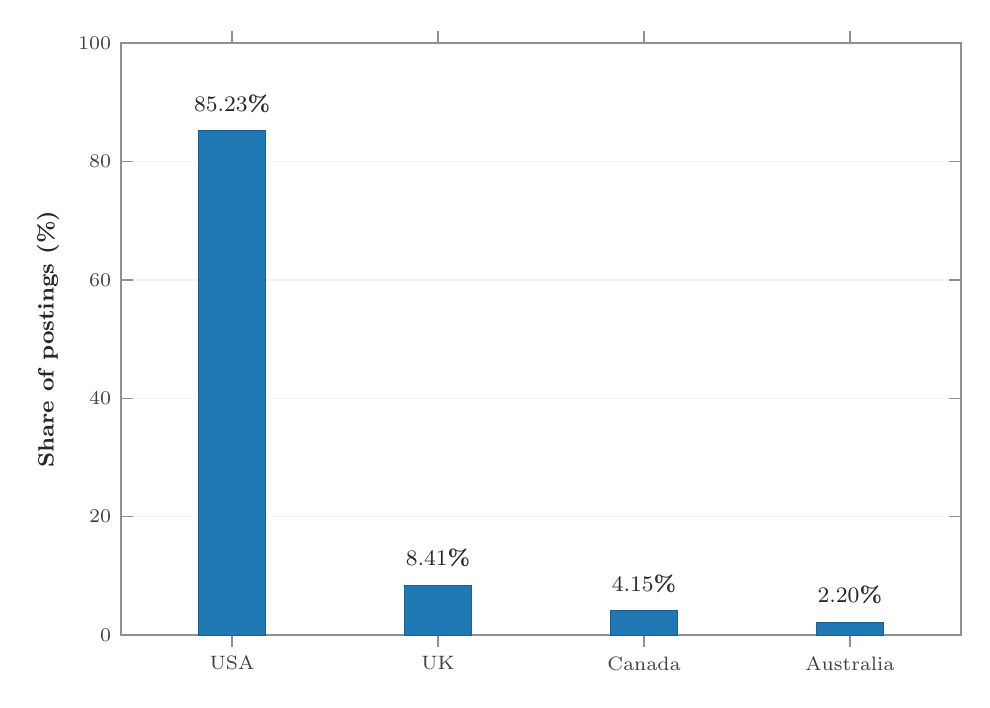
\begin{tikzpicture}
\begin{axis}[
  sg axis,
  ybar,
  bar width=24pt,
  width=0.88\linewidth,
  height=0.62\linewidth,
  symbolic x coords={USA,UK,Canada,Australia},
  xtick=data,
  ymin=0, ymax=100,
  ylabel={\textbf{Share of postings (\%)}},
  enlarge x limits=0.18,
  nodes near coords={\pgfmathprintnumber[fixed, zerofill=true, precision=2]{\pgfplotspointmeta}\%},
  every node near coord/.append style={font=\footnotesize\bfseries, color=black!85, yshift=3pt},
]
\addplot[sg bar=sgBlue] coordinates {
  (USA,85.23)(UK,8.41)(Canada,4.15)(Australia,2.20)
};
\end{axis}
\end{tikzpicture}%
}%
}

% ============================================================
% FIG 4a — Cohen's d (STAT01)
% ============================================================
\newcommand{\FigEffectSizes}{%
\resizebox{\linewidth}{!}{%
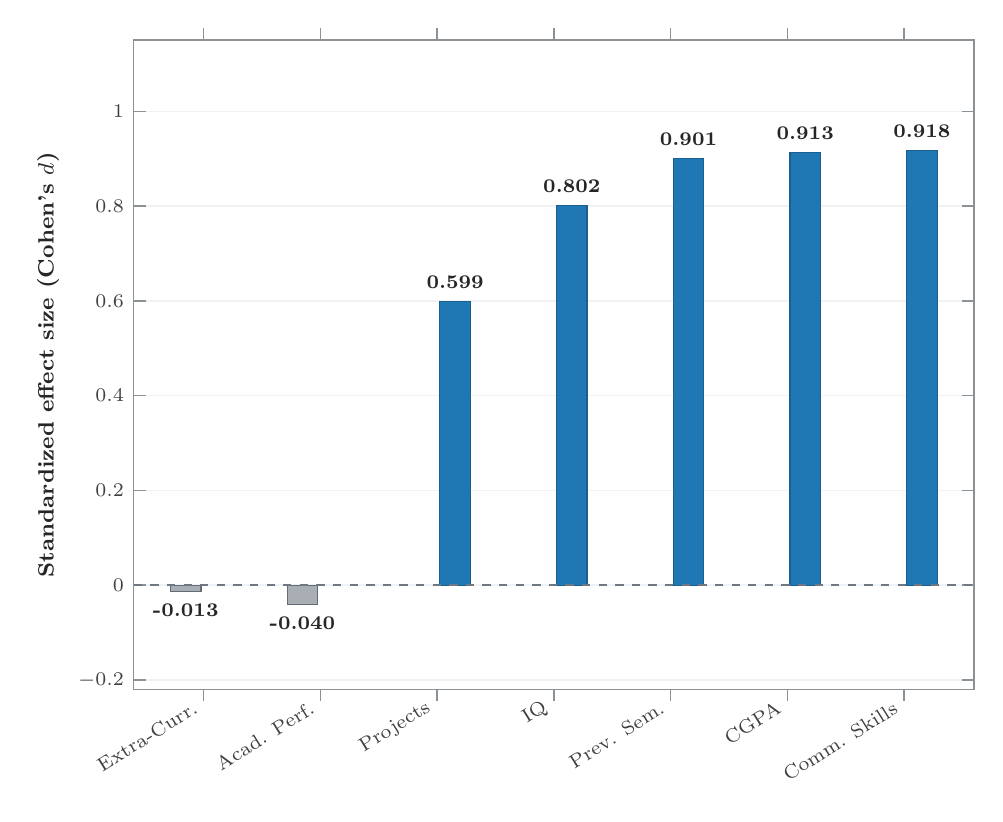
\begin{tikzpicture}
\begin{axis}[
  sg axis,
  ybar,
  bar width=11pt,
  width=0.88\linewidth,
  height=0.68\linewidth,
  symbolic x coords={ExtraCurr,AcadPerf,Projects,IQ,PrevSem,CGPA,CommSk},
  xtick={ExtraCurr,AcadPerf,Projects,IQ,PrevSem,CGPA,CommSk},
  xticklabels={Extra-Curr., Acad. Perf., Projects, IQ, Prev. Sem., CGPA, Comm. Skills},
  x tick label style={rotate=32, anchor=east, font=\scriptsize},
  ymin=-0.22, ymax=1.15,
  ylabel={\textbf{Standardized effect size (Cohen's $d$)}},
  enlarge x limits=0.10,
  point meta=explicit symbolic,
  nodes near coords,
]
\addplot[fill=sgGrey!60, draw=sgGrey!90!black, line width=0.4pt, every node near coord/.append style={font=\scriptsize\bfseries, color=black!85, anchor=north, yshift=-1pt}] coordinates {
  (ExtraCurr,-0.013) [-0.013]
  (AcadPerf,-0.040) [-0.040]
};
\addplot[fill=sgBlue, draw=sgBlue!80!black, line width=0.4pt, every node near coord/.append style={font=\scriptsize\bfseries, color=black!85, anchor=south, yshift=1pt}] coordinates {
  (Projects,0.599) [0.599]
  (IQ,0.802) [0.802]
  (PrevSem,0.901) [0.901]
  (CGPA,0.913) [0.913]
  (CommSk,0.918) [0.918]
};
\draw[dashed, sgGrey, line width=0.5pt] ({axis cs:ExtraCurr,0} -| {rel axis cs:0,0}) -- ({rel axis cs:1,0} |- {axis cs:ExtraCurr,0});
\end{axis}
\end{tikzpicture}%
}%
}

% ============================================================
% FIG 4b — Group means (STAT01)
% ============================================================
\newcommand{\FigMeans}{%
\resizebox{\linewidth}{!}{%
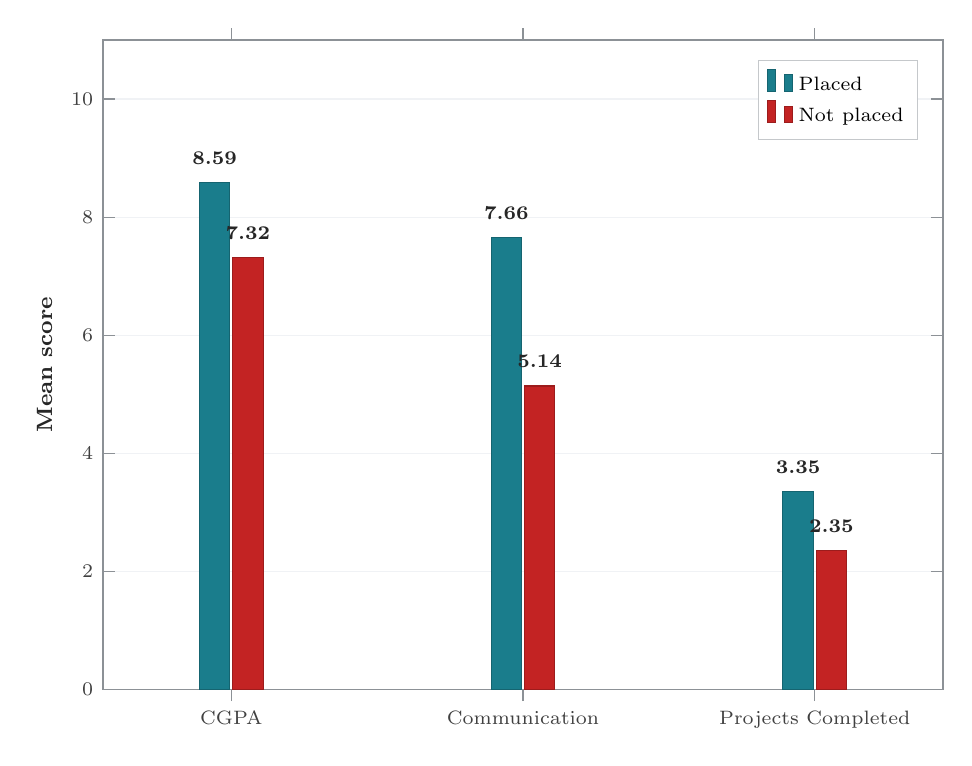
\begin{tikzpicture}
\begin{axis}[
  sg axis,
  ybar,
  bar width=11pt,
  width=0.88\linewidth,
  height=0.68\linewidth,
  symbolic x coords={CGPA,Comm,Projects},
  xtick=data,
  xticklabels={CGPA, Communication, Projects Completed},
  x tick label style={font=\scriptsize},
  ymin=0, ymax=11.0,
  ylabel={\textbf{Mean score}},
  enlarge x limits=0.22,
  legend pos=north east,
  point meta=explicit symbolic,
  nodes near coords,
  every node near coord/.append style={font=\scriptsize\bfseries, color=black!85, yshift=3pt},
]
\addplot[fill=sgTeal, draw=sgTeal!80!black, line width=0.4pt, bar shift=-6pt] coordinates {
  (CGPA,8.59) [8.59]
  (Comm,7.66) [7.66]
  (Projects,3.35) [3.35]
};
\addlegendentry{Placed}
\addplot[fill=sgRed, draw=sgRed!80!black, line width=0.4pt, bar shift=6pt] coordinates {
  (CGPA,7.32) [7.32]
  (Comm,5.14) [5.14]
  (Projects,2.35) [2.35]
};
\addlegendentry{Not placed}
\end{axis}
\end{tikzpicture}%
}%
}

% ============================================================
% FIG 5 — Internship employment rates (INTL01)
% ============================================================
\newcommand{\FigInternship}{%
\resizebox{0.88\linewidth}{!}{%
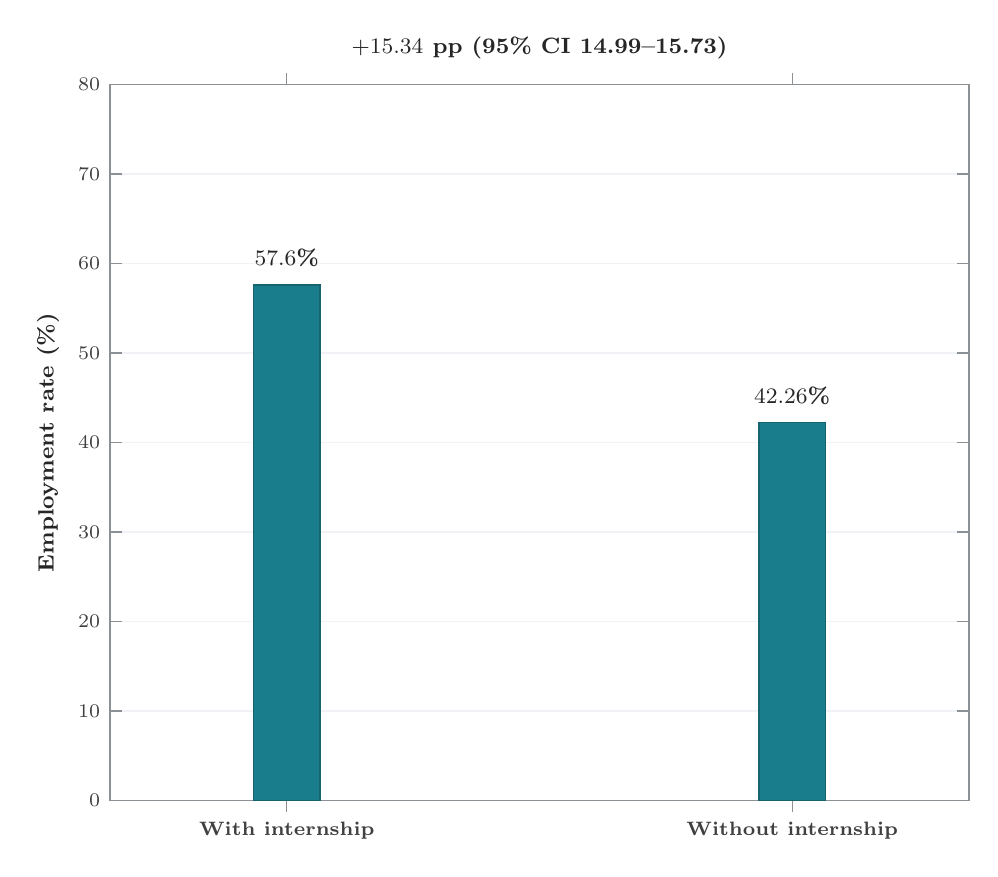
\begin{tikzpicture}
\begin{axis}[
  sg axis,
  ybar,
  bar width=24pt,
  width=0.90\linewidth,
  height=0.75\linewidth,
  symbolic x coords={With,Without},
  xtick={With,Without},
  xticklabels={With internship, Without internship},
  x tick label style={font=\scriptsize\bfseries},
  ymin=0, ymax=80,
  ylabel={\textbf{Employment rate (\%)}},
  enlarge x limits=0.35,
  nodes near coords={\pgfmathprintnumber[fixed, precision=2]{\pgfplotspointmeta}\%},
  every node near coord/.append style={font=\footnotesize\bfseries, color=black!85, yshift=3pt},
]
\addplot[fill=sgTeal, draw=sgTeal!80!black, line width=0.4pt] coordinates {
  (With,57.60)(Without,42.26)
};
\end{axis}
\node[font=\footnotesize\bfseries, text=black!85, anchor=south, align=center]
  at (current axis.north) [yshift=2mm]
  {$+15.34$ pp (95\% CI 14.99--15.73)};
\end{tikzpicture}%
}%
}
